\documentclass[conference]{IEEEtran}
\IEEEoverridecommandlockouts
\usepackage{cite}
\usepackage{amsmath,amssymb}
\usepackage{graphicx}
\usepackage{booktabs}
\usepackage{xcolor}
\usepackage{tikz}
\usetikzlibrary{positioning,calc}
\usepackage{url}
\usepackage[hidelinks]{hyperref}
\usepackage{microtype}
\graphicspath{{figures/}}
\renewcommand{\arraystretch}{1.08}
\newcommand{\eps}{\varepsilon}
\raggedbottom

\begin{document}

\title{Is It the Noise? Decomposing DP-SGD's Membership Protection and Auditing Data-Level Defences on a Small Clinical Dataset}

\author{\IEEEauthorblockN{Harshit Modi}
\IEEEauthorblockA{K. J. Somaiya School of Engineering, Somaiya Vidyavihar University, Mumbai, India\\
harshit.modi@somaiya.edu\\
\textit{Preprint, November 2026. Not peer reviewed.}}}

\maketitle

\begin{abstract}
Clinical prediction models trained on a few hundred patients can reveal who was in their training data. We audit diabetes classifiers trained on 192 records of the Pima Indians Diabetes dataset with three black-box membership inference attacks, up to the likelihood-ratio attack (LiRA) with 64 reference models, and ask where protection actually comes from. LiRA identifies 56.2\% of a Random Forest's training patients at a 1\% false-positive rate (FPR). Matched-recipe ablations split DP-SGD's effect on a neural network into shorter training, per-record clipping and calibrated noise. Under an average-case shadow-model attack, training length and clipping account for 53\% and 41\% of the drop in attack AUC ($p{=}0.002$ each), and the noise for 6\% ($p{=}0.85$). Under LiRA the noise accounts for 21\% and is significant: it lowers the true-positive rate at 1\% FPR from 2.0\% to 1.2\% (difference 0.8 points, 95\% CI 0.3--1.2). How much credit the noise receives therefore depends on the attack used to audit it. Under the same adversary, Mondrian $k$-anonymity and compressive projections leave a Random Forest's membership leakage largely intact (shadow-attack AUC 0.793 and about 0.70, from 0.814), and full-record local DP destroys utility. DP-SGD logistic regression at $\eps{=}4$ matches non-private accuracy (0.756 vs.\ 0.764, $p{=}0.41$) and exposes 1.2\% of members at 1\% FPR. On 253{,}680 CDC BRFSS records the cost of the noise falls to at most 0.003 ROC-AUC from 25{,}000 training records. Code, logs and 13 unit tests reproduce every number.
\end{abstract}

\begin{IEEEkeywords}
membership inference, differential privacy, DP-SGD, LiRA, k-anonymity, local differential privacy, compressive privacy, clinical machine learning
\end{IEEEkeywords}

\section{Introduction}
Clinical risk models are often trained on a few hundred patient records and then served through a prediction interface. A \emph{membership inference attack} (MIA) decides whether a given patient's record was in the training set~\cite{shokri2017,yeom2018}. For a disease cohort, membership is itself sensitive: it reveals that the person was a patient or a study participant. The defences that practitioners reach for act at different points of the data pipeline and promise different things: de-identification such as $k$-anonymity on the shared table~\cite{sweeney2002,lefevre2006}, local differential privacy (DP) at the patient~\cite{warner1965,kasiviswanathan2011}, compressive (dimension-reducing) releases of features~\cite{kung2017spm}, and central DP during training, usually DP-SGD~\cite{abadi2016,dwork2014}.

Two problems make it hard to tell which of these actually protects patients against membership inference. First, DP-SGD differs from ordinary training in more than its noise. It trains for few epochs, clips every per-record gradient, and samples lots at random. Overfitting drives leakage~\cite{yeom2018,shokri2017}, and short training and regularisation can reduce it on their own; a DP model's measured privacy therefore mixes the effect of the recipe with the effect of the mechanism. Second, defences are usually evaluated with different attacks and metrics, and average-case attack AUC hides the records that are most exposed~\cite{carlini2022,aerni2024}.

We address both on one small clinical task: diabetes prediction from 192 training records. One adversary audits every defence with three black-box attacks: a loss threshold~\cite{yeom2018}, a shadow-model attack~\cite{shokri2017} and online LiRA with 64 reference models~\cite{carlini2022}, reporting true-positive rates at low false-positive rates. Matched baselines add the ingredients of DP-SGD one at a time. We repeat every comparison on 10 random splits with paired tests, and we bootstrap LiRA at the record level. A second dataset, 253{,}680 CDC BRFSS survey records, separates small-data effects from the cost of privacy itself. Our contributions are:
\begin{itemize}
\item \textbf{A decomposition of DP-SGD's empirical protection.} Under a shadow-model attack, shorter training and clipping account for 94\% of the drop in attack AUC and the noise is not significant. Under LiRA, the noise accounts for 21\% and significantly lowers exposure at 1\% FPR. The credit the noise receives depends on the auditing attack.
\item \textbf{A same-adversary comparison of four defences} acting at different points of the pipeline: central DP, local DP, Mondrian $k$-anonymity, and compressive projections (PCA, discriminant component analysis and a privacy-aware variant). Defences on the data protect identity, the record or an attribute, but barely reduce model membership leakage.
\item \textbf{Evidence on model choice and data size.} On 192 records, DP logistic regression at $\eps{=}4$ is statistically indistinguishable in accuracy from its non-private counterpart. On BRFSS the cost of the noise vanishes from $n{=}25{,}000$, leaving a constant 0.02--0.03 ROC-AUC gap caused by the optimiser rather than by privacy.
\item \textbf{An open, tested implementation}: DP-SGD written from scratch with R\'enyi-DP accounting, all attacks and defences, 13 unit tests and a single script that regenerates every result.
\end{itemize}

\section{Related Work}
\textbf{Membership inference and its evaluation.} Shokri \emph{et al.}~\cite{shokri2017} introduced shadow-model MIAs; Yeom \emph{et al.}~\cite{yeom2018} tied leakage to overfitting and proposed the loss-threshold attack. Song and Mittal~\cite{song2021} showed that aggregate metrics underestimate risk and proposed per-record privacy risk scores. Carlini \emph{et al.}~\cite{carlini2022} argued that attacks must be judged by their true-positive rate at low false-positive rates and introduced LiRA, which fits per-example distributions of model confidence; RMIA~\cite{zarifzadeh2024} raises attack power further, especially when few reference models are available. Aerni \emph{et al.}~\cite{aerni2024} found that evaluations of heuristic defences underestimate leakage by an order of magnitude when they average over records, and that a well-tuned DP-SGD baseline beat every heuristic defence they studied. Tabular data raise their own evaluation challenges~\cite{pera2026}.

\textbf{DP-SGD in practice.} DP-SGD~\cite{abadi2016} clips per-example gradients and adds Gaussian noise; its cost is tracked with R\'enyi DP~\cite{mironov2017,mironov2019}. Measured leakage is usually far below what the guarantee permits~\cite{jayaraman2019}; auditing with crafted canaries under strong threat models can bring the two close~\cite{jagielski2020,nasr2023}. Tram\`er and Boneh~\cite{tramer2021} showed that under DP, linear models on good features beat end-to-end deep networks unless much more data is available. Practical guides~\cite{ponomareva2023} cover how to choose the clipping norm, batch size and training length under DP; tuning them on private data itself leaks~\cite{papernot2022}; adaptive clipping~\cite{andrew2021} avoids hand-tuning the norm. In health care, DP learning hurts minority groups and long-tailed records most~\cite{suriyakumar2021}. To our knowledge, prior work has not separated DP-SGD's measured protection into training length, clipping and noise with matched baselines and compared the split under an average-case attack and under LiRA, which is the focus of this paper.

\textbf{Defences that act on data.} $k$-anonymity~\cite{sweeney2002}, implemented here with Mondrian generalisation~\cite{lefevre2006}, protects a released table against linkage. Records are often re-identifiable from a few attributes~\cite{rocher2019}. Goldsteen \emph{et al.}~\cite{goldsteen2021} reported that model-guided anonymisation can resist MIAs about as well as DP; we test the more common case of generic Mondrian anonymisation of three quasi-identifiers. Randomised response~\cite{warner1965} is the canonical local DP mechanism~\cite{kasiviswanathan2011}; when only the label is sensitive, label DP is much cheaper than full DP~\cite{ghazi2021}. Compressive privacy~\cite{kung2017spm} releases a low-dimensional projection chosen for a utility task, e.g.\ discriminant component analysis (DCA)~\cite{kung2017dca}; RUCA~\cite{al2017ruca} and desensitised RDCA~\cite{filipowicz2017} additionally suppress a private attribute. Our privacy-aware DCA is a simple variant of that idea, not a new method.

\section{Threat Model and Defences}
\textbf{Setting.} A hospital trains a binary diabetes classifier on $n{=}192$ patient records and exposes its confidence scores through an API. Alternatively, it releases a projection $Z$ of its records instead of a model.

\textbf{Adversary.} The attacker's goal is to decide whether a target patient's record was in the training set. The attacker queries the model for confidence scores, knows the target's true label and the training recipe (Kerckhoffs's principle), and holds disjoint records from the same population (the \emph{shadow pool}). For LiRA we follow the evaluation game of Carlini \emph{et al.}~\cite{carlini2022}: reference models are trained on random halves of the whole 768-record population. This gives the attacker more information than a realistic outsider, so LiRA serves as an auditing tool and its numbers as conservative estimates of exposure. Against a released projection $Z$, the attacker also tries to infer a private attribute (age ${\geq}\,35$) and to reconstruct the record linearly, using the public projection matrix and its own data. White-box access to parameters or gradients, label-only interfaces, poisoning and linkage with outside data are out of scope; no re-identification is attempted.

\textbf{Defences.} Fig.~\ref{fig:pipeline} and Table~\ref{tab:defences} place the four defences in the pipeline. Only central DP bounds membership leakage for every attacker. For a balanced membership test, $(\eps,0)$-DP caps the accuracy of any attack at $e^{\eps}/(1+e^{\eps})$~\cite{kairouz2015}: 0.731 at $\eps{=}1$ and 0.982 at $\eps{=}4$.

\begin{figure*}[t]
\centering
\resizebox{0.97\textwidth}{!}{% Fig. 1: where each defence acts, and what the single adversary attacks (TikZ, vector).
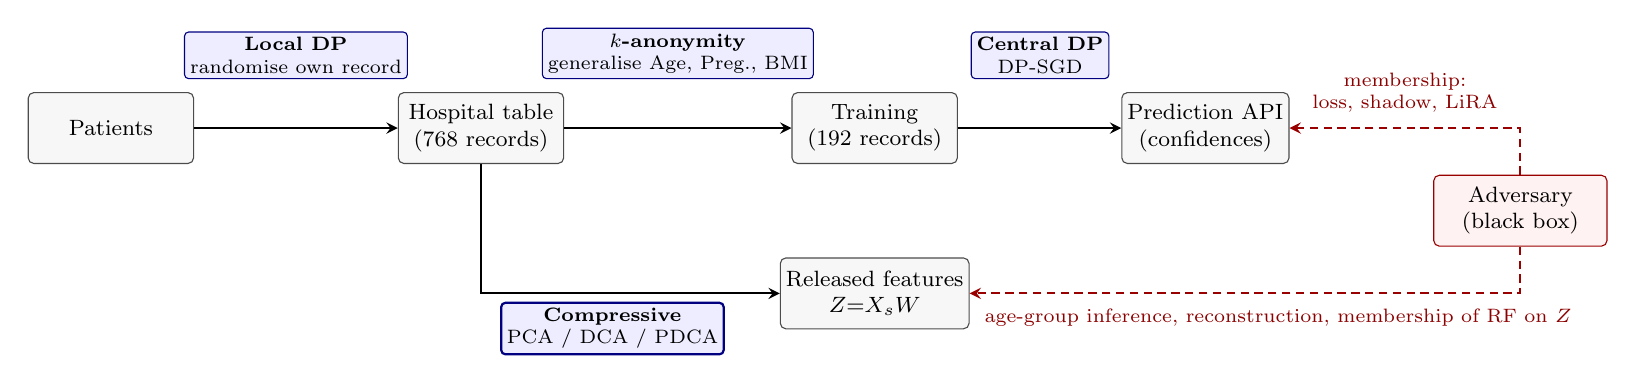
\begin{tikzpicture}[
  font=\footnotesize, >=stealth,
  box/.style={draw=black!70, rounded corners=2pt, fill=black!3, align=center, minimum height=9mm, minimum width=21mm, inner sep=2pt},
  def/.style={fill=blue!7, draw=blue!50!black, rounded corners=1.5pt, inner sep=2pt, align=center, font=\scriptsize},
  adv/.style={draw=red!60!black, fill=red!5, rounded corners=2pt, align=center, minimum height=9mm, minimum width=22mm, inner sep=2pt},
  att/.style={->, densely dashed, red!60!black, thick},
  lab/.style={font=\scriptsize, text=red!55!black, align=center}]
  \node[box] (pat) at (0,0) {Patients};
  \node[box] (tab) at (4.7,0) {Hospital table\\(768 records)};
  \node[box] (tr)  at (9.7,0) {Training\\(192 records)};
  \node[box] (api) at (13.9,0) {Prediction API\\(confidences)};
  \node[box] (z)   at (9.7,-2.1) {Released features\\$Z{=}X_sW$};
  \node[adv] (A)   at (17.9,-1.05) {Adversary\\(black box)};
  \draw[->, thick] (pat) -- (tab);
  \draw[->, thick] (tab) -- (tr);
  \draw[->, thick] (tr) -- (api);
  \node[def, anchor=south] at ($(pat)!0.5!(tab)+(0,0.62)$) {\textbf{Local DP}\\randomise own record};
  \node[def, anchor=south] at ($(tab)!0.5!(tr)+(0,0.62)$) {\textbf{$k$-anonymity}\\generalise Age, Preg., BMI};
  \node[def, anchor=south] at ($(tr)!0.5!(api)+(0,0.62)$) {\textbf{Central DP}\\DP-SGD};
  \draw[->, thick] (tab.south) |- node[def, pos=0.72, below=3pt] {\textbf{Compressive}\\PCA / DCA / PDCA} (z.west);
  \draw[att] (A.north) |- node[lab, pos=0.75, above=2pt] {membership:\\loss, shadow, LiRA} (api.east);
  \draw[att] (A.south) |- node[lab, pos=0.72, below=2pt] {age-group inference, reconstruction, membership of RF on $Z$} (z.east);
\end{tikzpicture}
}
\caption{Where each defence acts. One black-box adversary audits the model API with three membership attacks, and the released features with age-group inference, linear reconstruction and a membership attack on a Random Forest trained on $Z$.}
\label{fig:pipeline}
\end{figure*}

\begin{table}[t]
\centering\footnotesize
\caption{Defences compared under one adversary.}
\label{tab:defences}
\setlength{\tabcolsep}{3pt}
\begin{tabular}{@{}llll@{}}
\toprule
Defence & Acts on & Trusted party & Guarantee \\
\midrule
Central DP (DP-SGD) & training & hospital & $(\eps,\delta)$-DP, model \\
Local DP & each patient & none & $\eps$-LDP, report \\
Mondrian $k$-anonymity & shared table & hospital & syntactic \\
DCA / PDCA & released features & hospital & none (empirical) \\
\bottomrule
\end{tabular}
\end{table}

\section{Methods}
\subsection{Data and splits}
The Pima Indians Diabetes dataset~\cite{smith1988} has 768 records of women aged 21 or older, eight clinical features and a binary label (500 negative, 268 positive). We recode 652 physiologically impossible zeros in five columns as missing (Insulin 48.7\%, SkinThickness 29.6\% of records) and impute medians inside each model's pipeline. For each of 10 seeds, a stratified split assigns 384 records to the attacker's shadow pool, 192 to the target's training set (members) and 192 to a held-out set (non-members, also the test set). Standardisation is fitted on the training data.

\subsection{Models, DP-SGD and matched baselines}
We train logistic regression (LR; scikit-learn, $C{=}1$), a Random Forest (RF; 200 trees, unlimited depth) and a one-hidden-layer ReLU MLP (64 units, 641 parameters). The MLP and all DP variants are written in NumPy with closed-form per-record gradients. DP-SGD~\cite{abadi2016} takes steps
\begin{equation}
\tilde g_t=\frac{1}{qN}\Big(\sum_{i\in L_t} g_i\min\big(1,\tfrac{C}{\lVert g_i\rVert_2}\big)+\mathcal N(0,\sigma^2C^2 I)\Big),
\end{equation}
where each record joins the lot $L_t$ independently with probability $q{=}32/192$. We use 30 epochs (180 steps), learning rate 0.5 and $C{=}1$. The noise multiplier $\sigma$ is the smallest value for which a R\'enyi-DP accountant~\cite{mironov2017,mironov2019,dpaccounting} reports the target $\eps\in\{0.5,1,2,4,8\}$ at $\delta{=}10^{-5}$ ($\sigma{=}17.28$, 9.20, 4.97, 2.79 and 1.67). DP-LR is the same optimiser without a hidden layer (9 parameters) and uses the same $\sigma$. These settings were fixed in advance from a short trial on two splits and are not tuned per $\eps$.

To separate DP-SGD's ingredients we add them one at a time to a conventional non-private MLP (1000 epochs, learning rate 0.05, mini-batches of 32, trained until it fits the training set): (i)~\emph{matched}: the DP-SGD recipe of 30 epochs and learning rate 0.5 with shuffled mini-batches of 32, no clipping and no noise; (ii)~\emph{clip-only}: DP-SGD with $\sigma{=}0$; (iii)~DP-SGD at $\eps{=}4$. Step (ii) also replaces shuffled mini-batches with Poisson-sampled lots; we call it ``clipping'' for brevity. An L2-regularised MLP ($\lambda{=}10^{-2}$, 1000 epochs) is a non-DP alternative.

\subsection{Local DP, $k$-anonymity and compressive releases}
\textbf{Local DP.} Each patient randomises their own record before the hospital sees it. \emph{Label only}: randomised response~\cite{warner1965} keeps the diagnosis with probability $e^{\eps}/(1+e^{\eps})$. \emph{All attributes}: each feature is clipped to a public clinical range, rescaled to $[0,1]$ and perturbed with Laplace noise of scale $1/\eps_j$; the budget is split equally over the nine attributes, so each report is $\eps$-LDP by sequential composition. LR is trained on the noisy reports and predicts on clean inputs.

\textbf{$k$-anonymity.} Mondrian~\cite{lefevre2006} recursively splits the training records at the median of the widest normalised quasi-identifier (Age, Pregnancies, BMI) while both halves keep at least $k$ records, and replaces the quasi-identifiers by the range midpoints of their class. Test queries are routed through the same tree. We use $k\in\{2,5,10,25,50\}$ and report the normalised certainty penalty (NCP), the mean generalised range relative to the full range.

\textbf{Compressive releases.} The hospital releases $Z{=}X_sW$, where $X_s$ are the standardised training records. PCA keeps the $m\in\{1,\dots,4\}$ directions of largest variance. DCA~\cite{kung2017dca} keeps the leading generalised eigenvector of $S_B w=\lambda(S+\rho I)w$, with $S_B$ the between-class scatter of the diagnosis and $S$ the total scatter; a binary label gives one component. Privacy-aware DCA (PDCA) solves $(S_B^{\mathrm{dx}}-\beta S_B^{\mathrm{age}})\,w=\lambda(S+\rho I)\,w$, which keeps directions that separate the diagnosis but not the private age group, with $\beta\in\{1,3,10\}$ and $\rho{=}10^{-3}\,\mathrm{tr}(S)/8$. We measure utility with LR trained on $Z$; age-group inference with an LR attacker trained on the projected shadow pool; reconstruction as the $R^2$ of a linear map from $Z$ back to $X_s$, fitted on the shadow pool; and membership leakage of an RF trained on $Z$.

\subsection{Attacks}
The \emph{loss-threshold} attack~\cite{yeom2018} scores each record by its negative loss. The \emph{shadow-model} attack~\cite{shokri2017} trains 8 shadow models with the target's recipe on random halves of the shadow pool and fits a gradient-boosted attack classifier (100 trees, depth 2) on the confidence in the true label, its logit and the label. Both report AUC over the 192 members and 192 non-members of each split.

\emph{Online LiRA}~\cite{carlini2022} trains $K{=}64$ models of each configuration, each on a random half (384) of all 768 records, so every record is a member of about half of them. For target model $t$ and record $i$, it fits Gaussians to the logit confidence $\phi$ of the other 63 models that did and did not train on $i$ and scores $\Lambda_i=\log\mathcal N(\phi_t(i);\mu_{\mathrm{in}},\sigma^2_{\mathrm{in}})-\log\mathcal N(\phi_t(i);\mu_{\mathrm{out}},\sigma^2_{\mathrm{out}})$. Every model takes a turn as the target, giving $64\times768=49{,}152$ pooled decisions per configuration. We report the largest TPR at FPR $\leq1\%$ and $\leq0.1\%$, without interpolation. DP-SGD models in LiRA train on 384 records, so $\sigma$ is re-calibrated ($q{=}1/12$, 360 steps; $\sigma{=}6.53$, 2.04 and 1.29 for $\eps{=}1$, 4 and 8). LiRA results therefore describe models trained on 384 records, the other attacks models trained on 192.

\subsection{Statistics and correctness}
We report means over the 10 splits with 95\% $t$-intervals. Paired comparisons use two-sided Wilcoxon signed-rank tests paired by split; with 10 pairs the smallest attainable $p$ is 0.002. LiRA uses one population of 64 models per configuration, with the same membership masks in every configuration. Its 95\% confidence intervals come from 1{,}000 bootstrap resamples of the 768 records that keep each record's 64 decisions together, paired across configurations for differences. These intervals capture which records are sampled, not the randomness of retraining. Thirteen unit tests check per-record gradients against finite differences, the clipping bound on each update, the accountant calibration, randomised-response and Laplace statistics, the $k$-anonymity guarantee, the DCA and PDCA directions, and LiRA on a memorising and a constant model; all pass.

\subsection{Scaling study (BRFSS 2015)}
The CDC Diabetes Health Indicators dataset~\cite{brfss} has 253{,}680 survey records with 21 indicators (13.9\% positive). Features are min--max scaled with public codebook ranges, so the private pipeline uses no data-dependent preprocessing. For each of 3 seeds we hold out 20{,}000 stratified test records and draw a stratified training set of $n\in\{200, 1{,}000, 5{,}000, 25{,}000, 100{,}000\}$ from the rest. We train non-private LR, DP-SGD LR with $\sigma{=}0$ (\emph{no noise}), and DP-LR at $\eps\in\{4,1,0.5\}$ with $\delta{=}1/(10n)$, an expected lot of $\min(\max(32,n/50),2048)$, 20 epochs, learning rate 1.0 and $C{=}1$. This study measures utility only.

\section{Results}
\subsection{RQ1: How much do the models leak under a strong attack?}
LiRA exposes far more than the average-case attacks (Fig.~\ref{fig:lira}, Table~\ref{tab:lira}). At 1\% FPR it identifies 56.2\% (95\% CI 52.7--60.1) of the Random Forest's training patients, and 12.9\% at 0.1\% FPR; its best balanced accuracy is 0.895. The shadow attack, by comparison, scores the Random Forest at AUC 0.814. The non-private MLP exposes 10.7\% (9.2--12.5). Logistic regression and every DP-SGD model expose 1.0--1.3\% at 1\% FPR, against 1\% for random guessing. Their LiRA AUCs remain slightly above 0.5 (e.g.\ LR 0.530, 95\% CI 0.523--0.537), so a weak average-case signal remains without any high-confidence exposure.

The two models with the same test accuracy (0.764) differ most in leakage: LR and the Random Forest, whose generalisation gaps are 0.014 and 0.236. Model choice is itself a privacy decision.

\begin{figure*}[t]
\centering
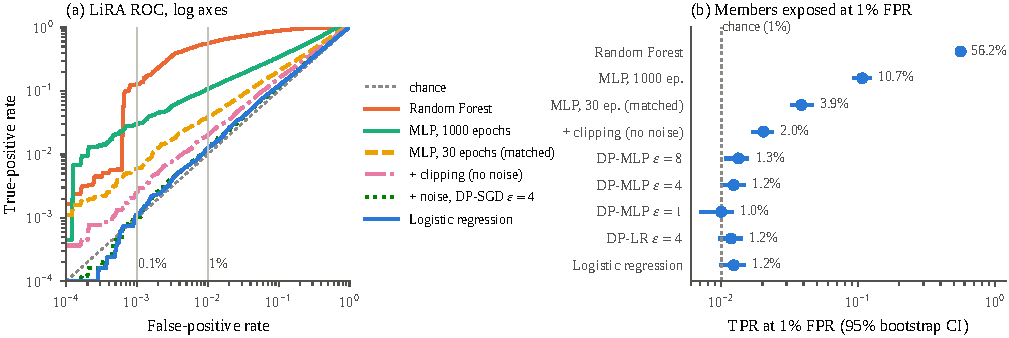
\includegraphics[width=\textwidth]{fig_lira.pdf}
\caption{LiRA audit on Pima (64 models per configuration, each trained on 384 records; 49{,}152 pooled decisions). (a) ROC curves on log axes; the low-FPR region on the left is what matters for privacy. Each added ingredient of DP-SGD moves the MLP's curve towards the diagonal. (b) Share of training records identified at 1\% FPR, with 95\% record-level bootstrap intervals; chance is 1\%.}
\label{fig:lira}
\end{figure*}

\begin{table}[t]
\centering\footnotesize
\caption{LiRA results (95\% record-level bootstrap intervals). Chance TPR equals the FPR.}
\label{tab:lira}
\setlength{\tabcolsep}{2.5pt}
\resizebox{\columnwidth}{!}{\begin{tabular}{@{}lccc@{}}
\toprule
Target model (384 records) & LiRA AUC & TPR@1\% (\%) & TPR@0.1\% (\%) \\
\midrule
Random Forest & 0.965 {\scriptsize[0.960, 0.969]} & 56.2 {\scriptsize[52.7, 60.1]} & 12.93 {\scriptsize[8.85, 19.01]} \\
MLP, 1000 epochs & 0.751 {\scriptsize[0.736, 0.765]} & 10.7 {\scriptsize[9.2, 12.5]} & 3.00 {\scriptsize[1.95, 4.38]} \\
MLP, 30 epochs (matched) & 0.624 {\scriptsize[0.613, 0.635]} & 3.9 {\scriptsize[3.2, 4.7]} & 0.61 {\scriptsize[0.33, 0.92]} \\
+ clipping, no noise & 0.575 {\scriptsize[0.567, 0.583]} & 2.0 {\scriptsize[1.7, 2.4]} & 0.25 {\scriptsize[0.13, 0.40]} \\
DP-SGD MLP, $\varepsilon{=}8$ & 0.545 {\scriptsize[0.537, 0.552]} & 1.3 {\scriptsize[1.1, 1.6]} & 0.09 {\scriptsize[0.05, 0.17]} \\
DP-SGD MLP, $\varepsilon{=}4$ & 0.530 {\scriptsize[0.522, 0.537]} & 1.2 {\scriptsize[1.0, 1.5]} & 0.09 {\scriptsize[0.04, 0.18]} \\
DP-SGD MLP, $\varepsilon{=}1$ & 0.507 {\scriptsize[0.499, 0.513]} & 1.0 {\scriptsize[0.7, 1.2]} & 0.09 {\scriptsize[0.03, 0.21]} \\
DP-SGD LR, $\varepsilon{=}4$ & 0.520 {\scriptsize[0.513, 0.527]} & 1.2 {\scriptsize[1.0, 1.4]} & 0.09 {\scriptsize[0.05, 0.16]} \\
Logistic regression & 0.530 {\scriptsize[0.523, 0.537]} & 1.2 {\scriptsize[1.0, 1.5]} & 0.11 {\scriptsize[0.04, 0.21]} \\
\bottomrule
\end{tabular}
}
\end{table}

\subsection{RQ2: Where does DP-SGD's protection come from?}
Table~\ref{tab:decomp} and Fig.~\ref{fig:decomp} add DP-SGD's ingredients one at a time. Against the shadow attack, cutting training from 1000 to 30 epochs lowers attack AUC from 0.713 to 0.612 ($p{=}0.002$), and per-record clipping lowers it to 0.534 ($p{=}0.002$). Adding noise for $\eps{=}4$ brings it to 0.522, a difference this attack cannot resolve ($p{=}0.846$). Training length and clipping account for 53\% and 41\% of the total drop of 0.191, and the noise for 6\%. The loss-threshold attack agrees ($p{=}0.002$, 0.002 and 0.105).

LiRA divides the credit differently. The same three steps lower LiRA AUC by 0.127, 0.049 and 0.045, so the noise accounts for 21\% of the total drop of 0.221, as much as clipping, and its 95\% interval (0.037--0.053) excludes zero. At 1\% FPR the exposure falls from 10.7\% to 3.9\%, 2.0\% and finally 1.2\%; the noise step removes 0.8 points (95\% CI 0.3--1.2). Clipping alone therefore still leaves twice-chance exposure. The noise removes most of what remains, and it is also what carries the formal guarantee.

Ordinary regularisation does not replace the mechanism. An L2-regularised MLP reaches similar accuracy to DP-SGD at $\eps{=}4$ (0.752 vs.\ 0.735, $p{=}0.195$) but leaks more under the shadow attack (0.586 vs.\ 0.522, $p{=}0.002$) and under LiRA (AUC 0.625 vs.\ 0.530). Along the decomposition, accuracy rises from 0.706 to 0.728 with shorter training and to 0.756 with clipping, then falls to 0.735 with the noise (Fig.~\ref{fig:decomp}).

\begin{table}[t]
\centering\footnotesize
\caption{Decomposing DP-SGD (MLP). Change in attack AUC as each ingredient is added. Shadow and loss: 192-record models, 10 splits, Wilcoxon $p$. LiRA: 384-record models, paired record-level bootstrap.}
\label{tab:decomp}
\setlength{\tabcolsep}{2.5pt}
\resizebox{\columnwidth}{!}{\begin{tabular}{@{}lccc@{}}
\toprule
Step added & Shadow AUC & Loss AUC & LiRA AUC \\
 & {\scriptsize $\Delta$ ($p$, Wilcoxon)} & {\scriptsize $\Delta$ ($p$)} & {\scriptsize $\Delta$ [95\% CI]} \\
\midrule
Shorter training (1000$\to$30 epochs) & $-$0.102 (0.002) & $-$0.036 (0.002) & $-$0.127 {\scriptsize[0.118, 0.135]} \\
Per-record clipping ($C{=}1$) & $-$0.078 (0.002) & $-$0.043 (0.002) & $-$0.049 {\scriptsize[0.040, 0.058]} \\
Gaussian noise ($\varepsilon{=}4$) & $-$0.011 (0.846) & $-$0.009 (0.105) & $-$0.045 {\scriptsize[0.037, 0.053]} \\
\midrule
Total (MLP $\to$ DP-SGD, $\varepsilon{=}4$) & $-$0.191 (0.002) & $-$0.088 & $-$0.221 \\
\bottomrule
\end{tabular}
}
\end{table}

\begin{figure}[t]
\centering
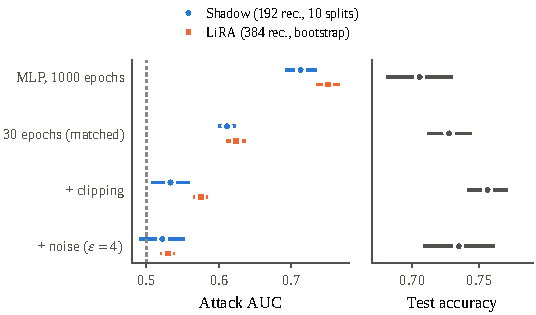
\includegraphics[width=\columnwidth]{fig_decomposition.pdf}
\caption{Each row adds one ingredient of DP-SGD to the non-private MLP. Left: attack AUC under the shadow attack (mean and 95\% CI over 10 splits) and LiRA (95\% bootstrap CI). Right: test accuracy. The noise step is invisible to the shadow attack but clear under LiRA.}
\label{fig:decomp}
\end{figure}

\subsection{RQ3: What does central DP cost, and for which model?}
On 192 records the simpler model is the better private model (Fig.~\ref{fig:frontier}, Table~\ref{tab:grid}). DP-LR beats the DP-MLP at $\eps{=}1$ (accuracy 0.726 vs.\ 0.642, $p{=}0.004$) and at $\eps{=}4$ (0.756 vs.\ 0.735, $p{=}0.027$). At $\eps{=}4$, DP-LR is statistically indistinguishable in accuracy from non-private LR (0.756 vs.\ 0.764, $p{=}0.410$), with ROC-AUC 0.824 vs.\ 0.828 and higher recall (0.607 vs.\ 0.543). Its LiRA AUC is 0.520 and it exposes 1.2\% of members at 1\% FPR. Every DP-SGD model sits at shadow-attack AUC 0.478--0.526. The DP-MLP needs $\eps\geq4$ to be useful; at $\eps\leq1$ its accuracy falls to 0.612--0.642.

\begin{figure}[t]
\centering
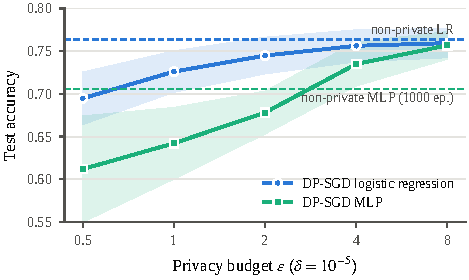
\includegraphics[width=\columnwidth]{fig_frontier.pdf}
\caption{Central DP on Pima: test accuracy against $\eps$ for DP-SGD logistic regression and the DP-SGD MLP (mean and 95\% CI over 10 splits). Dashed lines: non-private references.}
\label{fig:frontier}
\end{figure}

\textbf{Hyperparameters.} At a fixed $\eps{=}4$, with $\sigma$ re-calibrated for each setting, the DP-MLP's accuracy ranges from 0.646 ($C{=}5$) to 0.759 ($C{=}0.5$) (Table~\ref{tab:sens}). A large clipping norm wastes the budget on noise. A very small one biases every gradient: at $C{=}0.1$ ROC-AUC stays at 0.816 but F1 drops to 0.420. Fewer epochs need less noise for the same $\eps$ (10 epochs: $\sigma{=}1.817$, accuracy 0.758). The setting we fixed in advance was not the best one, but choosing the best cell on test data would itself leak~\cite{papernot2022}, so headline results keep the pre-set configuration.

\begin{table}[t]
\centering\footnotesize
\caption{DP-SGD MLP at a fixed $\eps{=}4$: one setting varied at a time, $\sigma$ re-calibrated (mean$\pm$95\% CI, 10 splits).}
\label{tab:sens}
\setlength{\tabcolsep}{3pt}
\begin{tabular}{@{}lcccc@{}}
\toprule
Setting ($\varepsilon{=}4$) & $\sigma$ & Accuracy & F1 & Shadow AUC \\
\midrule
$C{=}0.1$, 30 epochs & 2.785 & 0.721$\pm$0.026 & 0.420 & 0.514 \\
$C{=}0.5$, 30 epochs & 2.785 & 0.759$\pm$0.017 & 0.616 & 0.509 \\
$C{=}1$, 30 epochs (used) & 2.785 & 0.735$\pm$0.026 & 0.592 & 0.522 \\
$C{=}2$, 30 epochs & 2.785 & 0.685$\pm$0.019 & 0.522 & 0.532 \\
$C{=}5$, 30 epochs & 2.785 & 0.646$\pm$0.029 & 0.485 & 0.535 \\
$C{=}1$, 10 epochs & 1.817 & 0.758$\pm$0.018 & 0.607 & 0.514 \\
$C{=}1$, 60 epochs & 3.802 & 0.712$\pm$0.017 & 0.535 & 0.518 \\
$C{=}1$, 120 epochs & 5.278 & 0.692$\pm$0.027 & 0.559 & 0.525 \\
\bottomrule
\end{tabular}

\end{table}

\textbf{Data size.} On BRFSS (Fig.~\ref{fig:scaling}, Table~\ref{tab:scaling}), comparing DP-LR with the same optimiser without noise isolates the cost of the noise. At $\eps{=}4$ it is 0.057 ROC-AUC at $n{=}200$ and 0.004 at $n{=}5{,}000$. From $n{=}25{,}000$ it is at most 0.003 even at $\eps{=}0.5$. The optimiser itself stays 0.020--0.031 below non-private LR at every $n$, with or without noise; this gap comes from clipping and a fixed 20-epoch budget, not from privacy. Small-$n$ results depend on the setup: on Pima, DP-LR at $\eps{=}4$ nearly matched non-private ROC-AUC at $n{=}192$, while on BRFSS at $n{=}200$ it does not (0.666 vs.\ 0.743). The two settings differ in feature scaling, class balance (34.9\% vs.\ 13.9\% positive), learning rate and $\delta$. With 3 seeds, intervals at $n\leq1{,}000$ are wide.

\begin{figure}[t]
\centering
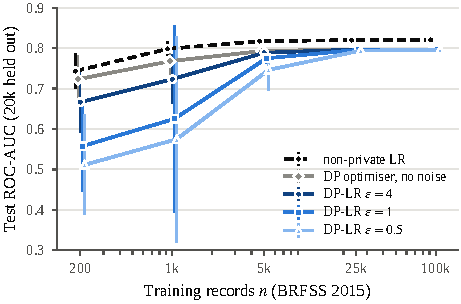
\includegraphics[width=\columnwidth]{fig_scaling.pdf}
\caption{BRFSS 2015: ROC-AUC on 20{,}000 held-out records against training-set size (mean and 95\% $t$-interval over 3 seeds). The gap between the grey line (same optimiser, no noise) and the blue lines is the cost of the noise.}
\label{fig:scaling}
\end{figure}

\begin{table}[t]
\centering\footnotesize
\caption{BRFSS ROC-AUC (3 seeds). In brackets: DP-LR minus the same optimiser without noise, i.e.\ the cost of the noise.}
\label{tab:scaling}
\setlength{\tabcolsep}{3pt}
\resizebox{\columnwidth}{!}{\begin{tabular}{@{}rccccc@{}}
\toprule
$n$ & Non-private & No noise & $\varepsilon{=}4$ & $\varepsilon{=}1$ & $\varepsilon{=}0.5$ \\
\midrule
200 & 0.743 & 0.723 & 0.666 {\scriptsize($-$0.057)} & 0.558 {\scriptsize($-$0.165)} & 0.511 {\scriptsize($-$0.212)} \\
1,000 & 0.798 & 0.767 & 0.723 {\scriptsize($-$0.044)} & 0.625 {\scriptsize($-$0.142)} & 0.575 {\scriptsize($-$0.193)} \\
5,000 & 0.817 & 0.793 & 0.788 {\scriptsize($-$0.004)} & 0.775 {\scriptsize($-$0.018)} & 0.746 {\scriptsize($-$0.047)} \\
25,000 & 0.820 & 0.797 & 0.797 {\scriptsize(0.000)} & 0.796 {\scriptsize($-$0.001)} & 0.794 {\scriptsize($-$0.003)} \\
100,000 & 0.820 & 0.796 & 0.796 {\scriptsize(0.000)} & 0.796 {\scriptsize(0.000)} & 0.796 {\scriptsize(0.000)} \\
\bottomrule
\end{tabular}
}
\end{table}

\begin{table*}[t]
\centering\footnotesize
\caption{All Pima configurations: utility on the 192 non-members and shadow-attack AUC (mean$\pm$95\% CI over 10 splits). Gap: train minus test accuracy.}
\label{tab:grid}
\begin{tabular}{@{}llccccccc@{}}
\toprule
Model & $\varepsilon$ & $\sigma$ & Accuracy & Recall & F1 & ROC-AUC & Gap & Shadow AUC \\
\midrule
Logistic regression & -- & -- & 0.764$\pm$0.018 & 0.543 & 0.616 & 0.828 & 0.014 & 0.498$\pm$0.024 \\
Random Forest & -- & -- & 0.764$\pm$0.017 & 0.558 & 0.622 & 0.814 & 0.236 & 0.814$\pm$0.012 \\
MLP, 1000 epochs & -- & -- & 0.706$\pm$0.024 & 0.546 & 0.564 & 0.761 & 0.291 & 0.713$\pm$0.020 \\
MLP + L2 & -- & -- & 0.752$\pm$0.021 & 0.555 & 0.609 & 0.812 & 0.131 & 0.586$\pm$0.025 \\
MLP, 30 ep.\ (matched) & -- & -- & 0.728$\pm$0.016 & 0.557 & 0.583 & 0.784 & 0.161 & 0.612$\pm$0.010 \\
+ clipping, $\sigma{=}0$ & $\infty$ & 0 & 0.756$\pm$0.014 & 0.557 & 0.612 & 0.822 & 0.060 & 0.534$\pm$0.025 \\
\midrule
DP-SGD MLP & 0.5 & 17.28 & 0.612$\pm$0.062 & 0.442 & 0.442 & 0.591 & 0.023 & 0.511$\pm$0.023 \\
DP-SGD MLP & 1 & 9.20 & 0.642$\pm$0.042 & 0.479 & 0.478 & 0.645 & 0.032 & 0.519$\pm$0.017 \\
DP-SGD MLP & 2 & 4.97 & 0.678$\pm$0.025 & 0.510 & 0.520 & 0.716 & 0.057 & 0.526$\pm$0.023 \\
DP-SGD MLP & 4 & 2.79 & 0.735$\pm$0.026 & 0.558 & 0.592 & 0.785 & 0.048 & 0.522$\pm$0.029 \\
DP-SGD MLP & 8 & 1.67 & 0.757$\pm$0.016 & 0.584 & 0.624 & 0.813 & 0.047 & 0.524$\pm$0.017 \\
\midrule
DP-SGD LR & 0.5 & 17.28 & 0.695$\pm$0.031 & 0.618 & 0.586 & 0.749 & 0.017 & 0.478$\pm$0.024 \\
DP-SGD LR & 1 & 9.20 & 0.726$\pm$0.024 & 0.622 & 0.614 & 0.788 & 0.018 & 0.499$\pm$0.032 \\
DP-SGD LR & 2 & 4.97 & 0.745$\pm$0.022 & 0.610 & 0.626 & 0.813 & 0.024 & 0.495$\pm$0.032 \\
DP-SGD LR & 4 & 2.79 & 0.756$\pm$0.019 & 0.607 & 0.635 & 0.824 & 0.014 & 0.498$\pm$0.015 \\
DP-SGD LR & 8 & 1.67 & 0.759$\pm$0.017 & 0.591 & 0.631 & 0.827 & 0.013 & 0.510$\pm$0.016 \\
\bottomrule
\end{tabular}

\end{table*}

\subsection{RQ4: What does local DP cost compared with central DP?}
Removing trust in the hospital is expensive on small data (Fig.~\ref{fig:dataside}a). With the budget split over nine attributes, each attribute receives $\eps/9$, which at $\eps{=}4$ is 0.44 and means Laplace noise with a standard deviation about 3.2 times the attribute's range. Trained on such reports, LR collapses towards a constant predictor. At $\eps\leq2$ it predicts a single class in every split. At $\eps{=}8$ and 16 its recall is at most 0.03 in every split, so its accuracy (0.652) is essentially that of predicting ``no diabetes'' for everyone (0.651). Its ROC-AUC at $\eps{=}16$ (0.727) is below central DP-LR at $\eps{=}0.5$ (0.749), a 32 times smaller budget.

Randomising only the diagnosis is nearly free at $\eps\geq4$ (accuracy 0.762 vs.\ 0.764), because symmetric label noise below a flip rate of 0.5 weakens the signal without moving the Bayes decision boundary; at $\eps{=}4$ the flip rate is 1.8\%. At $\eps{=}1$ (flip rate 26.9\%) accuracy falls to 0.708, below central DP-LR (0.726). Label-only randomisation protects the diagnosis but leaves the eight clinical features unprotected and gives no membership guarantee for the trained model.

\subsection{RQ5: Do data-level defences reduce model membership leakage?}
\textbf{$k$-anonymity.} The shared table is highly identifying: 95.4\% of the 768 records are unique on Age, Pregnancies and BMI alone, and 97.9--100\% of each 192-record training set. Mondrian anonymisation removes that: every class has at least $k$ records, so no training record is unique on the quasi-identifiers. At $k{=}50$, 67.5\% of the quasi-identifier detail is generalised away (NCP 0.675). Yet the Random Forest's shadow-attack AUC moves only from 0.814 to 0.805 at $k{=}2$, 0.793 at $k{=}5$ ($p{=}0.002$) and 0.794 at $k{=}50$ ($p{=}0.010$), while its accuracy drops from 0.764 to 0.745 ($k{=}5$, $p{=}0.020$) and 0.738 ($k{=}50$, $p{=}0.006$) (Fig.~\ref{fig:dataside}b). The drop is detectable but leaves the model highly attackable. $k$-anonymity hides identity, whereas membership inference reads the model's confidence on the full record, including the five clinical features that generalisation leaves untouched. Logistic regression does not leak to begin with, and anonymisation changes neither its leakage nor its accuracy ($p\geq0.156$).

\textbf{Compressive releases.} A single DCA component keeps the diagnostic signal of all eight features (Table~\ref{tab:cp}, Fig.~\ref{fig:dataside}c): accuracy 0.764 and ROC-AUC 0.827 vs.\ 0.828, while a linear attacker reconstructs only $R^2{=}0.21$ of the record. PCA with one component keeps less of the diagnosis (ROC-AUC 0.796) and more of the age group (inference AUC 0.814 vs.\ 0.751 for DCA), because it keeps variance rather than the utility task. PDCA steers the component away from age: at $\beta{=}10$ age-group inference falls to chance (AUC 0.504; attacker accuracy 0.632 against a majority rate of 0.637) for 1.2 points of accuracy. Neither projection is a membership defence. A Random Forest trained on any one-dimensional DCA or PDCA release still reaches shadow-attack AUC 0.696--0.705 at accuracy 0.678--0.702.

\begin{figure*}[t]
\centering
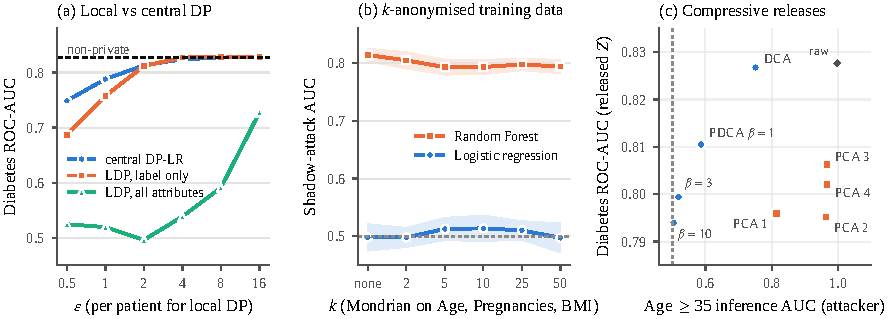
\includegraphics[width=\textwidth]{fig_dataside.pdf}
\caption{Defences that do not act on training. (a) Local vs.\ central DP for logistic regression (ROC-AUC on clean test records, mean over 10 splits). (b) Shadow-attack AUC of models trained on Mondrian-$k$-anonymised data (mean and 95\% CI); dashed: chance. (c) Released projections: diabetes ROC-AUC of LR on $Z$ against the attacker's age-group inference AUC; upper left is best.}
\label{fig:dataside}
\end{figure*}

\begin{table}[t]
\centering\footnotesize
\caption{Compressive releases (mean, $\pm$95\% CI over 10 splits). Age AUC: attacker infers age ${\geq}35$ from $Z$. $R^2$: linear reconstruction of the standardised record.}
\label{tab:cp}
\setlength{\tabcolsep}{2pt}
\resizebox{\columnwidth}{!}{\begin{tabular}{@{}lccccc@{}}
\toprule
Release $Z$ & Acc.\ (LR on $Z$) & ROC-AUC & Age AUC & $R^2$ & RF shadow AUC \\
\midrule
Raw features (8-D) & 0.764$\pm$0.018 & 0.828 & 0.999$\pm$0.001 & 1.00 & 0.814$\pm$0.012 \\
PCA, $m{=}4$ & 0.732$\pm$0.020 & 0.802 & 0.967$\pm$0.009 & 0.72 & 0.778$\pm$0.014 \\
PCA, $m{=}1$ & 0.722$\pm$0.019 & 0.796 & 0.814$\pm$0.033 & 0.27 & 0.718$\pm$0.023 \\
DCA, $m{=}1$ & 0.764$\pm$0.016 & 0.827 & 0.751$\pm$0.031 & 0.21 & 0.696$\pm$0.016 \\
PDCA, $\beta{=}1$ & 0.766$\pm$0.021 & 0.810 & 0.587$\pm$0.016 & 0.18 & 0.701$\pm$0.016 \\
PDCA, $\beta{=}3$ & 0.755$\pm$0.020 & 0.799 & 0.519$\pm$0.028 & 0.17 & 0.700$\pm$0.018 \\
PDCA, $\beta{=}10$ & 0.752$\pm$0.018 & 0.794 & 0.504$\pm$0.017 & 0.16 & 0.705$\pm$0.019 \\
\bottomrule
\end{tabular}
}
\end{table}

\section{Discussion}
\begin{table*}[t]
\centering\footnotesize
\caption{Every defence under the same adversary (mean over 10 splits; LiRA TPR at 1\% FPR where audited, chance 1\%). $^\dagger$Utility is LR on $Z$; leakage is an RF trained on $Z$.}
\label{tab:compare}
\begin{tabular}{@{}llccccl@{}}
\toprule
Mechanism & Setting & Acc. & ROC-AUC & Shadow AUC & LiRA TPR@1\% & Formal guarantee \\
\midrule
None & Logistic regression & 0.764 & 0.828 & 0.498 & 1.2\% & none \\
 & Random Forest & 0.764 & 0.814 & 0.814 & 56.2\% & none \\
\addlinespace[2pt]
Central DP & DP-SGD LR, $\varepsilon{=}4$ & 0.756 & 0.824 & 0.498 & 1.2\% & $(4,10^{-5})$-DP \\
 & DP-SGD LR, $\varepsilon{=}1$ & 0.726 & 0.788 & 0.499 & -- & $(1,10^{-5})$-DP \\
 & DP-SGD MLP, $\varepsilon{=}4$ & 0.735 & 0.785 & 0.522 & 1.2\% & $(4,10^{-5})$-DP \\
\addlinespace[2pt]
Local DP & Label only (RR), $\varepsilon{=}4$ & 0.762 & 0.827 & 0.506 & -- & 4-LDP, label \\
 & All attributes, $\varepsilon{=}16$ & 0.652 & 0.727 & 0.514 & -- & 16-LDP, record \\
\addlinespace[2pt]
$k$-anonymity & $k{=}5$ + Random Forest & 0.745 & 0.796 & 0.793 & -- & syntactic \\
 & $k{=}5$ + LR & 0.757 & 0.820 & 0.513 & -- & syntactic \\
\addlinespace[2pt]
Compressive & DCA, $m{=}1$ (RF on $Z$)$^\dagger$ & 0.764 & 0.827 & 0.696 & -- & none (empirical) \\
 & PDCA, $\beta{=}10$ (RF on $Z$)$^\dagger$ & 0.752 & 0.794 & 0.705 & -- & none (empirical) \\
\bottomrule
\end{tabular}

\end{table*}

Table~\ref{tab:compare} places the best tested setting of each defence next to the non-private baselines.

\textbf{The auditing attack decides how much the noise is worth.} An evaluator using a shadow-model attack would conclude that DP-SGD's noise is unnecessary, since a short, clipped training run reaches the same attack AUC. LiRA reverses that conclusion for the records that matter: clipping alone leaves twice-chance exposure at 1\% FPR (2.0\%), and the noise removes most of the excess (1.2\%, against 1\% for guessing). The shadow attack cannot see this because it learns one global decision rule from confidence features, and 192 non-members per split cannot resolve false-positive rates near 1\%. Privacy audits should therefore report TPR at low FPR from per-example attacks, as Carlini \emph{et al.}~\cite{carlini2022} and Aerni \emph{et al.}~\cite{aerni2024} argue; our decomposition shows a concrete case where the average-case conclusion would be wrong.

\textbf{Measured leakage is far below the formal cap.} At $\eps{=}4$ the guarantee allows a balanced attack accuracy of 0.982, whereas LiRA's best balanced accuracy is 0.52. As in earlier evaluations~\cite{jayaraman2019}, moderate $\eps$ protects well in practice. A strong guarantee itself requires $\eps\leq1$, and on 192 records only DP logistic regression stays useful there.

\textbf{Match the defence to the threat.} $k$-anonymity protects a published table against linkage, and compressive releases protect the record and a chosen attribute. Neither changes what a model trained on the data reveals about membership. Combining them with DP is the natural fix when both a table and a model are released. Our $k$-anonymity result differs from Goldsteen \emph{et al.}~\cite{goldsteen2021}, whose model-guided anonymisation reduced MIA success; generic Mondrian on three quasi-identifiers leaves the features a forest memorises untouched.

\textbf{Simplicity is a privacy asset.} The most accurate non-private model (LR, tied with the RF at 0.764) leaks almost nothing; the RF leaks the most at the same accuracy. Under DP, the 9-parameter model beats the 641-parameter one, as Tram\`er and Boneh~\cite{tramer2021} found for image tasks. For a hospital publishing a risk model trained on a few hundred records, our evidence supports DP-SGD logistic regression at $\eps$ between 1 and 4 with $\delta{=}10^{-5}$, audited with LiRA at low FPR.

\section{Limitations}
\textbf{One small dataset, one population.} All privacy results rest on Pima: 768 records from women aged 21 or older of a single Indigenous community, collected decades ago with heavy hidden missingness. The public release does not document the consent or governance of the original study; Radin~\cite{radin2017} traces how these records came to circulate as a benchmark. BRFSS tests only how utility scales with $n$; we ran no attacks on it, and it has only 3 seeds.

\textbf{Dependent splits and multiple tests.} The 10 splits reuse the same 768 records, so they are not independent and our $t$-intervals and $p$-values are somewhat optimistic. Of the 14 pre-specified paired tests, those at $p{=}0.002$ survive a Bonferroni threshold of 0.0036; DP-LR vs.\ DP-MLP at $\eps{=}1$ ($p{=}0.004$) and $\eps{=}4$ ($p{=}0.027$) do not.

\textbf{LiRA uncertainty and training size.} Each LiRA configuration is one population of 64 models; our bootstrap intervals cover the choice of records but not retraining randomness. TPR at 0.1\% FPR rests on about 25 false positives per configuration. LiRA targets models trained on 384 records while the other attacks target 192-record models, so the two decompositions are not on identical models.

\textbf{Attacker scope.} We consider black-box adversaries that see confidence scores. White-box, gradient-based and label-only attacks, canary-based auditing~\cite{nasr2023}, and stronger attacks such as RMIA~\cite{zarifzadeh2024} may change the numbers. Attribute inference and reconstruction from projections use linear attackers and one private attribute.

\textbf{Privacy accounting outside $\eps$.} On Pima, imputation medians and standardisation statistics are computed without DP, and the hyperparameters were chosen non-privately on two splits; neither cost is counted in $\eps$~\cite{papernot2022}. The BRFSS pipeline avoids the first issue by using public ranges. The ``clipping'' step of the decomposition also switches to Poisson sampling, and the Random Forest, the leakiest model, has no private variant here.

\section{Conclusion}
On a small clinical dataset, most of DP-SGD's measured protection against membership inference comes from its recipe of short, clipped training. The calibrated noise matters for the most exposed records, but only a per-example attack such as LiRA can see it. Defences that act on the data protect identity, records and attributes, not membership in a trained model. Among the configurations we audited with LiRA, DP-SGD logistic regression at $\eps{=}4$ was the one that combined non-private accuracy, near-chance exposure at 1\% FPR and a formal guarantee. We recommend that clinical privacy audits report TPR at low FPR from a per-example attack, compare DP against matched non-private recipes, and treat model choice as part of the privacy design.

\section*{Reproducibility statement}
All code, per-split logs and result tables are released with this preprint, together with the source and SHA-256 hash of both datasets. A single script (\texttt{run\_all.sh}) runs the 13 unit tests and seven experiments and regenerates the figures in about 30 minutes on a 2-core CPU without a GPU. The record-level LiRA bootstrap and every figure and table in this paper are generated by scripts that read the result files directly; a claim checker compares the numbers quoted in the text against those files. All randomness is seeded; a full rerun of the seven experiments in a fresh environment reproduced every result file exactly. Dependencies: NumPy, pandas, scikit-learn, SciPy, matplotlib and Google's \texttt{dp-accounting}~\cite{dpaccounting}.

\section*{Ethics statement}
Both datasets are public and de-identified. We attack only models we trained, attempt no linkage or re-identification, and report only aggregate results. The Pima data come from a long-running epidemiological study in the Gila River Indian Community~\cite{radin2017}; we use them because they are a standard small clinical benchmark, and we note that their reuse raises questions of Indigenous data governance~\cite{carroll2020} that public benchmark copies do not resolve.

\section*{Acknowledgment}
This work grew out of coursework in Security and Privacy for Machine Learning at K.~J.~Somaiya School of Engineering. In line with IEEE policy on AI-generated content, the author discloses that Claude (Anthropic) was used to help write and debug code, to build the bootstrap analysis, figures and tables from the result files, and to draft and edit the text of all sections. The author reviewed and verified all code, results and text and takes full responsibility for the content.

\bibliographystyle{IEEEtran}
\bibliography{refs}

\end{document}
